\subsection{Behaviour}
A QActor is an active (autonomous) entity that runs in parallel with the other actors defined in the same or in other contexts. The behaviour of a QActor can be expressed as a Moore Finite State Machine (M-FSM). Each state of the M-FSM can be expressed by a \textbf{Plan} which is composed of a sequence of \textbf{actions}.
Here are the finite state machines of our system:
\begin{figure}[h]
	\centering
	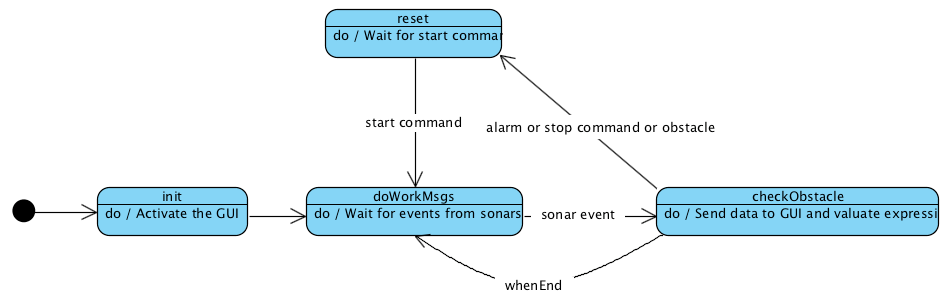
\includegraphics[width=\linewidth]{radargui.png}
	\caption{FSM for the radargui actor.}
\end{figure}
\begin{figure}[h]
	\centering
	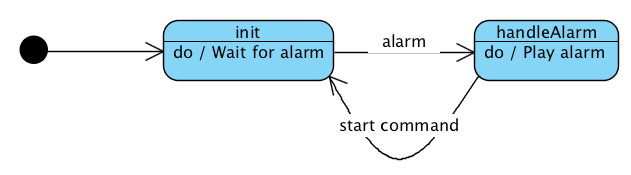
\includegraphics[width=9cm]{alarmhandler.png}
	\caption{FSM for the alarmhandler actor.}
\end{figure}
\begin{figure}[h]
	\centering
	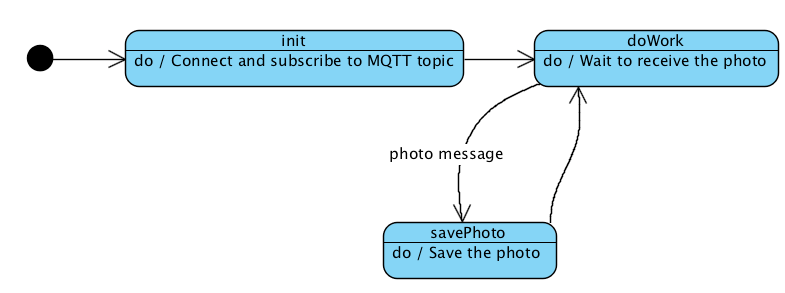
\includegraphics[width=9cm]{photoreceiver.png}
	\caption{FSM for the photoreceiver actor.}
\end{figure}
\begin{figure}[h]
	\centering
	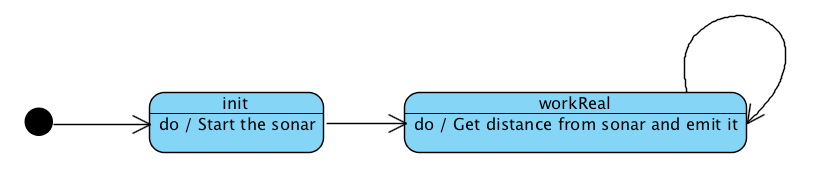
\includegraphics[width=9cm]{sensorsonar.png}
	\caption{FSM for the sensorsonar actor.}
\end{figure}
\begin{figure}[h]
	\centering
	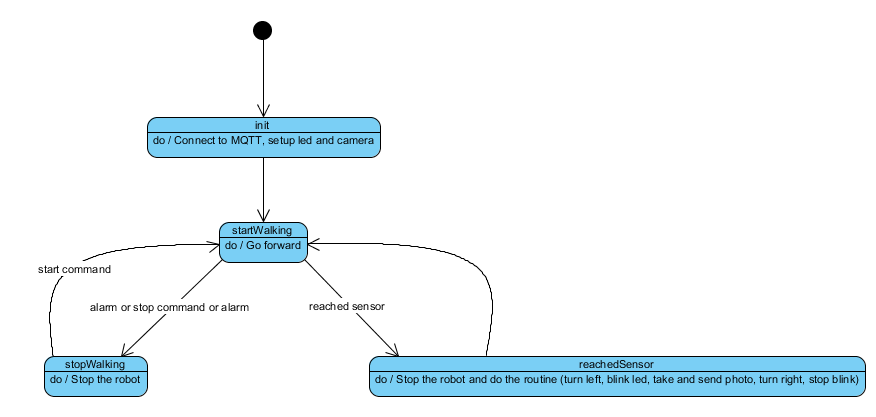
\includegraphics[width=\linewidth]{robotactor.png}
	\caption{FSM for the robot actor.}
\end{figure}
\clearpage